\chapter{Vizualizace skrze programovatelný logický automat}
V této kapitole se nachází popis jednotlivých částí ovládání instalace skrze PLC firmy TECO - CP-2007 \cite{TECO}, které obsahuje knihovny pro práci s KNX/IP \cite{KNXlib} a MQTT \cite{MQTTlib} a dále integrovaný webový server pro vizualizaci \cite{WebMaker}. Všechny tyto části jsou podrobněji rozvedeny v následujících podkapitolách.
Ovládání a vizualizace instalace je možné provádět i skrze PLC jiných výrobců za předpokladu, že mají implementované knihovny pro komunikace KNX/IP a MQTT. PLC výrobce TECO bylo vybráno kvůli jeho specializaci na domácí automatizaci, dostupnosti a ceně.
\section{CP - 2007}
Jedná se základní modul řídícího systému Foxtrot v provední s jednojádrovým procesorem ARMv7 o frekvenci 792MHz a databoxem o velikosti 128kB, který je vyroben pro přichycení na DIN Lištu. Obsahuje 2 ethernet porty, 2 sériové porty, 15 vstupů z nichž je 14 univerzálních a 1 galvanicky oddělený digitální, 15 výstupů z nichž je 11 releových a 4 analogové. Dále pak obsahuje 2 sloty na rozšiřující moduly. \cite{TECO}

\begin{figure}[!ht]
    \begin{center}
        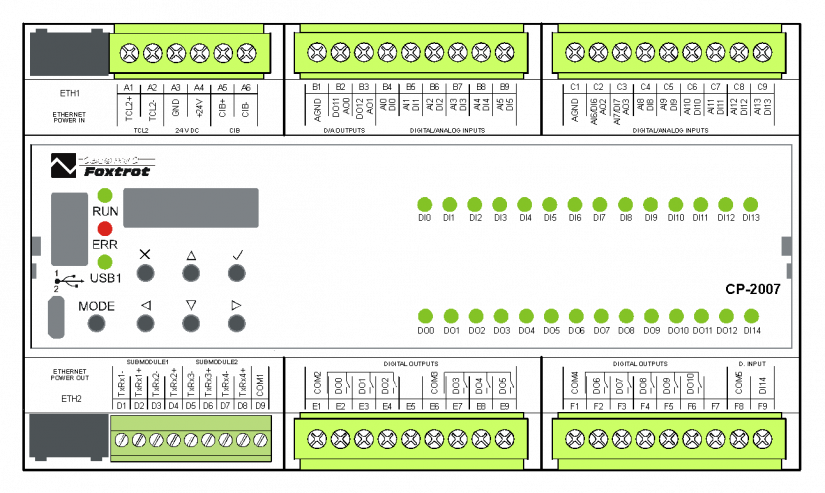
\includegraphics[scale=0.7]{obrazky/CP-2007.png}
    \end{center}
    \caption[CP-2007 \cite{TECO}]{CP-2007 \cite{TECO}}
    \label{fig:CP-2007}
\end{figure}

\section{Mosaic}
Ovládání instalace bylo realizováno v programovacím prostředí společnosti TECO - Mosaic, které je určeno pro programování PLC. Toto prostředí nabízí široké spektrum funkcí a nástrojů pro programování, vizualizaci a správu projektů \cite{Mosaic}: 

\begin{itemize}
    \item \textbf{Programovací jazyky dle IEC 61131-3 \cite{IEC61131-3}:}
        \begin{itemize}
            \item Ladder Diagram (LD)
            \item Function Block Diagram (FBD)
            \item Structured Text (ST)
            \item Instruction List (IL)
            \item Sequential Function Chart (SFC)
            \item Continuous Function Chart (CFC)
        \end{itemize}
    \item \textbf{Simulační nástroje:}
        \begin{itemize}
            \item Simulátor PLC
            \item Simulátor panelu
        \end{itemize}
    \item \textbf{Archivační nástroje:}
        \begin{itemize}
            \item Datalogger
            \item Správce souborů projektu
            \item Správce knihoven
        \end{itemize}
    \item \textbf{Nástroje pro tvorbu vizualizace:}
        \begin{itemize}
            \item WebMaker
            \item PanelMaker
            \item GraphMaker
        \end{itemize}
    \item \textbf{Inženýrské a pomocné nástroje:}
        \begin{itemize}
        \item Mapování uživatelských registrů
        \item I/O konfigurátor
        \item PID Maker
        \item PLCnet Manažer
        \item LangMan (jazykový manažer)
        \item Debuger
        \item IEC Manažer
        \item Asistent 16 → 32 (Převod 16bitového projektu na 32bitový)
        \item Texty KEY2 (Správa textových řetězců pro operační panely KEY2)
        \item Import KNX (Import konfigurace KNX IP BAOS z csv souboru)
        \item Firmware Updater
        \item Project Loader
        \item Set PLC IP
        \item Mosaic Updater
        \item Jazyk prostředí / IDE Language
    \end{itemize}
\end{itemize}

\subsection{Ovládací prvky}
Pro ovládání instalace byly vytvořeny funkční bloky, které byly poté použity v realizaci logiky programu:

\begin{itemize}
    \item \textbf{Základní funkční bloky:}
        \begin{itemize}
            \item fbKNXVisuBool - Ovládání binárních signálů skrze vizualizaci
            \item fbKNXShutters - Ovládání žaluzií skrze vizualizaci
            \item fbRoomTempMod - Modelovaní teploty místnosti v závislosti na parametrech a vstupech z topení a klimatizace (měření teploty z panelu bude neměnné - neumožní demonstraci změny teploty)
        \end{itemize}
    \item \textbf{Funkční bloky jednotlivých místností:}
        \begin{itemize}
            \item fbLivRoom - Ovládání obývacího pokoje a simulace teploty
            \item fbKitch - Ovládání kuchyně a simulace teploty
            \item fbBath - Ovládání koupelny a simulace teploty
            \item fbOutz - Ovládání vstupu a měření venkovní teploty (teplota z panelu) \newline
        \end{itemize}
\end{itemize}

\noindent Níže jsou uvedeny definice jednotlivých funkční bloků, které byly použity pro ovládání a vizualizaci instalace. Pro jejich realizaci byly použity jazyky CFC a ST.

\subsubsection{fbKNXVisuBool}
\begin{lstlisting}[language=ST]
FUNCTION_BLOCK fbKNXVisuBool
  VAR_INPUT
    IN           : BOOL R_EDGE; //Světlo ON Vizu
    OFF          : BOOL R_EDGE; //Světlo OFF Vizu
    FB           : BOOL; //KNX Světlo Feedback
  END_VAR
  VAR_OUTPUT
    OUT_CMD      : DT_CMD_BOOL; //KNX CMD
    OUT          : BOOL; //Visu hodnota
  END_VAR
  VAR
    TP_TIME : TIME := T#1S; //KNX CMD délka
    RS1 : RS;
    TP1 : TP;
  END_VAR

\end{lstlisting}

\begin{figure}[!ht]
    \begin{center}
        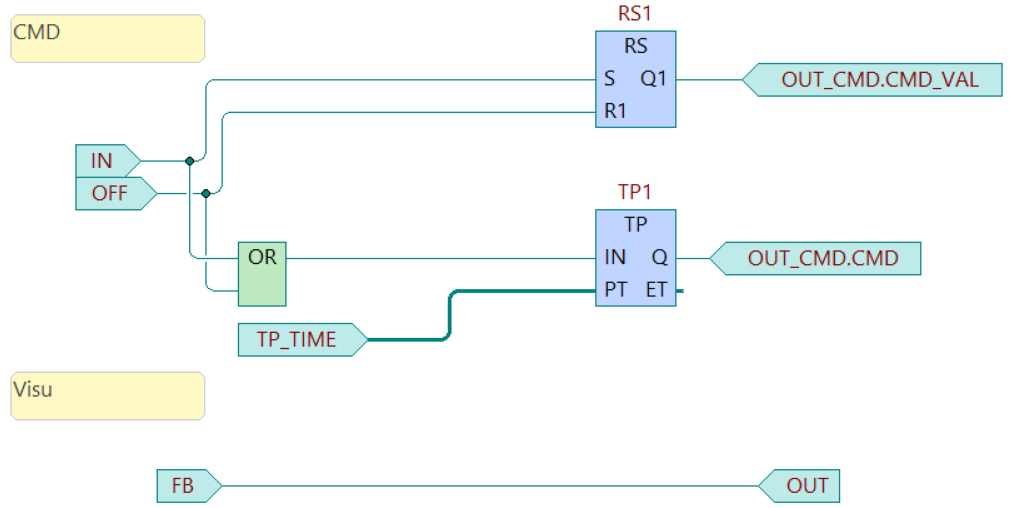
\includegraphics[scale=0.5]{obrazky/fbKNXVisuBool.png}
    \end{center}
    \caption[fbKNXVisuBool]{fbKNXVisuBool}
    \label{fig:fbKNXVisuBool}
\end{figure}
\newpage
\subsubsection{fbKNXShutters}
\begin{lstlisting}[language=ST]
    FUNCTION_BLOCK fbKNXShutters
    VAR_INPUT
      UP           : BOOL R_EDGE; //Rolety nahorů Vizu
      DOWN         : BOOL R_EDGE; //Rolety dolů Vizu
      UP_STEP      : BOOL; //Rolety nahorů krok Vizu
      DOWN_STEP    : BOOL; //Rolety dolů krok Vizu
      FB_UP        : BOOL; //KNX Rolety Feedback nahorů
      FB_DOWN      : BOOL; //KNX Rolety Feedback dolů
    END_VAR
    VAR_OUTPUT
      OUT_CMD      : DT_CMD_BOOL; //KNX CMD
      OUT_STEP_CMD : DT_CMD_BOOL; //KNX CMD krok
      OUT_UP       : BOOL; //Visu nahorů
      OUT_DOWN     : BOOL; //Visu dolů
    END_VAR
    VAR
      TP_TIME : TIME := T#1S; //KNX CMD délka
      RS1 : RS;
      TP1 : TP;
      RS2 : RS;
    END_VAR
\end{lstlisting}

\begin{figure}[!ht]
    \begin{center}
        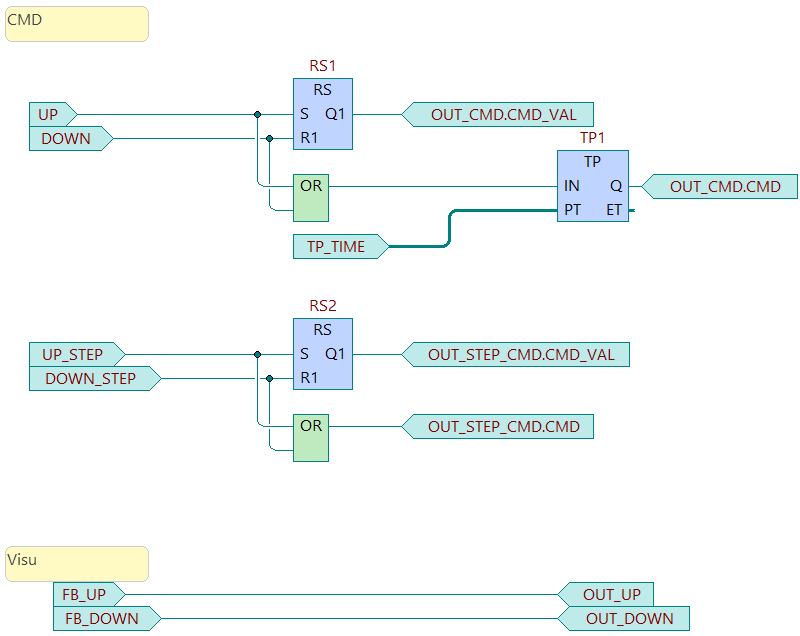
\includegraphics[scale=0.7]{obrazky/fbKNXShutters.png}
    \end{center}
    \caption[fbKNXShutters]{fbKNXShutters}
    \label{fig:fbKNXShutters}
\end{figure}
\subsubsection{fbRoomTempMod}
Na modelování teploty místnosti byl vytvořen jednoduchý matematický model, který měl za úkol zobrazit změnu v závislosti na působení topení a klimatizace.
Uvažujeme, že místnost je kvádr o rozměrech specifikovaných uživatelským vstupem Tento kvádr je naplněný vzduchem, který má určitou váhu, ze které lze vypočítat energie potřebná ke změně o teploty o 1 °C.

\begin{equation}
    V = a \cdot b \cdot c
    \label{eq:objem}
\end{equation}
\begin{equation}
    m = \rho \cdot V
    \label{eq:hmotnost}
\end{equation}
\begin{equation}
    Q = m \cdot c_p
    \label{eq:energie}
\end{equation}
\noindent\textit{Kde:}
\begin{itemize}
    \item $V$ - objem vzduchu v místnosti [m$^3$]
    \item $a$, $b$, $c$ - rozměry místnosti [m]
    \item $m$ - hmotnost vzduchu v místnosti [kg]
    \item $\rho$ - hustota vzduchu při tlaku jedné atmosféry a teplotě 20 °C - 1.204 [kg/m$^3$]
    \item $Q$ - energie potřebná ke změně teploty o 1 °C [J]
    \item $c_p$ - měrná tepelná kapacita vzduchu - 1005 [J$\cdot$kg$^{-1}\cdot$K$^{-1}$] \newline
\end{itemize}
\noindent Dále uvažujeme obal kvádru (stěny, podlahu a strop) s různými tloušťkami a tepelnými vodivostmi. Pro zjednodušení výpočtu se předpokládá, že dveře a okna místnosti nemají rozdílný vliv oproti stěnám a tudíž tepelný tok zůstává na celé ploše strany stejný a směr toku závisí pouze na poměru teplot na obou stranách zdi. Dále je předpoklad nulových teplot z jiných směrů. Také budeme předpokládat, že materiál bude všude stejný a to cihla. 

\begin{equation}
    S = a \cdot b
    \label{eq:plocha}
\end{equation}
\begin{equation}
    \Delta T = T_{in} - T_{out}
    \label{eq:rozdil_teplot}
\end{equation}
\begin{equation}
    \phi _{Strana} = \frac{\lambda \cdot S \cdot \Delta T}{c}
    \label{eq:tepelny_tok}
\end{equation}
\noindent\textit{Kde:}
\begin{itemize}
    \item $S$ - plocha strany [m$^2$]
    \item $a$, $b$, $c$ - rozměry strany [m]
    \item $\Delta T$ - rozdíl teploty na obou stranách strany [°C]
    \item $T_{in}$ - teplota uvnitř místnosti [°C]
    \item $T_{out}$ - teplota venku [°C]
    \item $\phi _{Strana}$ - tepelný tok [W]
    \item $\lambda$ - tepelná vodivost cihly - 0.4 [W$\cdot$m$^{-1}\cdot$K$^{-1}$] \newline
\end{itemize}
\noindent Další součástí simulace je topení a klimatizace, které jsou dodávány pouze jako binární signály. Pro jednoduché modelování byly vytvořeny funkce růstu (logaritmický) a poklesu (exponenciální) výkonu. Tyto funkce jsou zobrazeny na Obr. \ref{fig:simulace_funkce} Dále k těmto rovnicím byly vytvořeny korekční členy, které ovlivňují rychlost funkcí a tudíž více přiblížily chování funkcí více realitě.

\begin{equation}
    f_{Růst}(t) = \frac{ln(1 + k_{Růst} \cdot t)}{ln(1 + k_{Růst} \cdot t_{MaxRůst})} \cdot y_{Max}
    \label{eq:funkce_rust}
\end{equation} 
\begin{equation}
    k_{Růst} = \frac{t_{MaxRise}}{t_{80}}
    \label{eq:k_rust}
\end{equation}
\begin{equation}
    f_{Pokles}(t) = \frac{y}{e^{k_{Pokles} \cdot t}}
    \label{eq:funkce_pokles}
\end{equation}
\begin{equation}
    k_{Pokles} = \frac{\frac{y_{max}}{\varepsilon}}{t_{MaxPokles}}
    \label{eq:k_pokles}
\end{equation}
\newpage
\noindent\textit{Kde:}
\begin{itemize}
    \item $f_{Růst}(x)$ - funkce růstu výkonu [W]
    \item $k_{Růst}$ - korekční člen pro pokles [-]
    \item $t$ - čas [s]
    \item $t_{MaxRůst}$ - maximální čas růstu výkonu [s]
    \item $y_{Max}$ - maximální výkon [W]
    \item $t_{80}$ - čas potřebný k dosažení 80\% výkonu [s]
    \item $f_{Pokles}(x)$ - funkce poklesu výkonu [W]
    \item $k_{Pokles}$ - korekční člen pro růst [-] 
    \item $y$ - aktuální výkon [W]
    \item $\varepsilon$ - cílová hodnota pod kterou se výkon musí dostat [W]
    \item $t_{MaxPokles}$ - maximální čas poklesu výkonu [s]
\end{itemize}
\begin{figure}[!ht]
    \begin{center}
        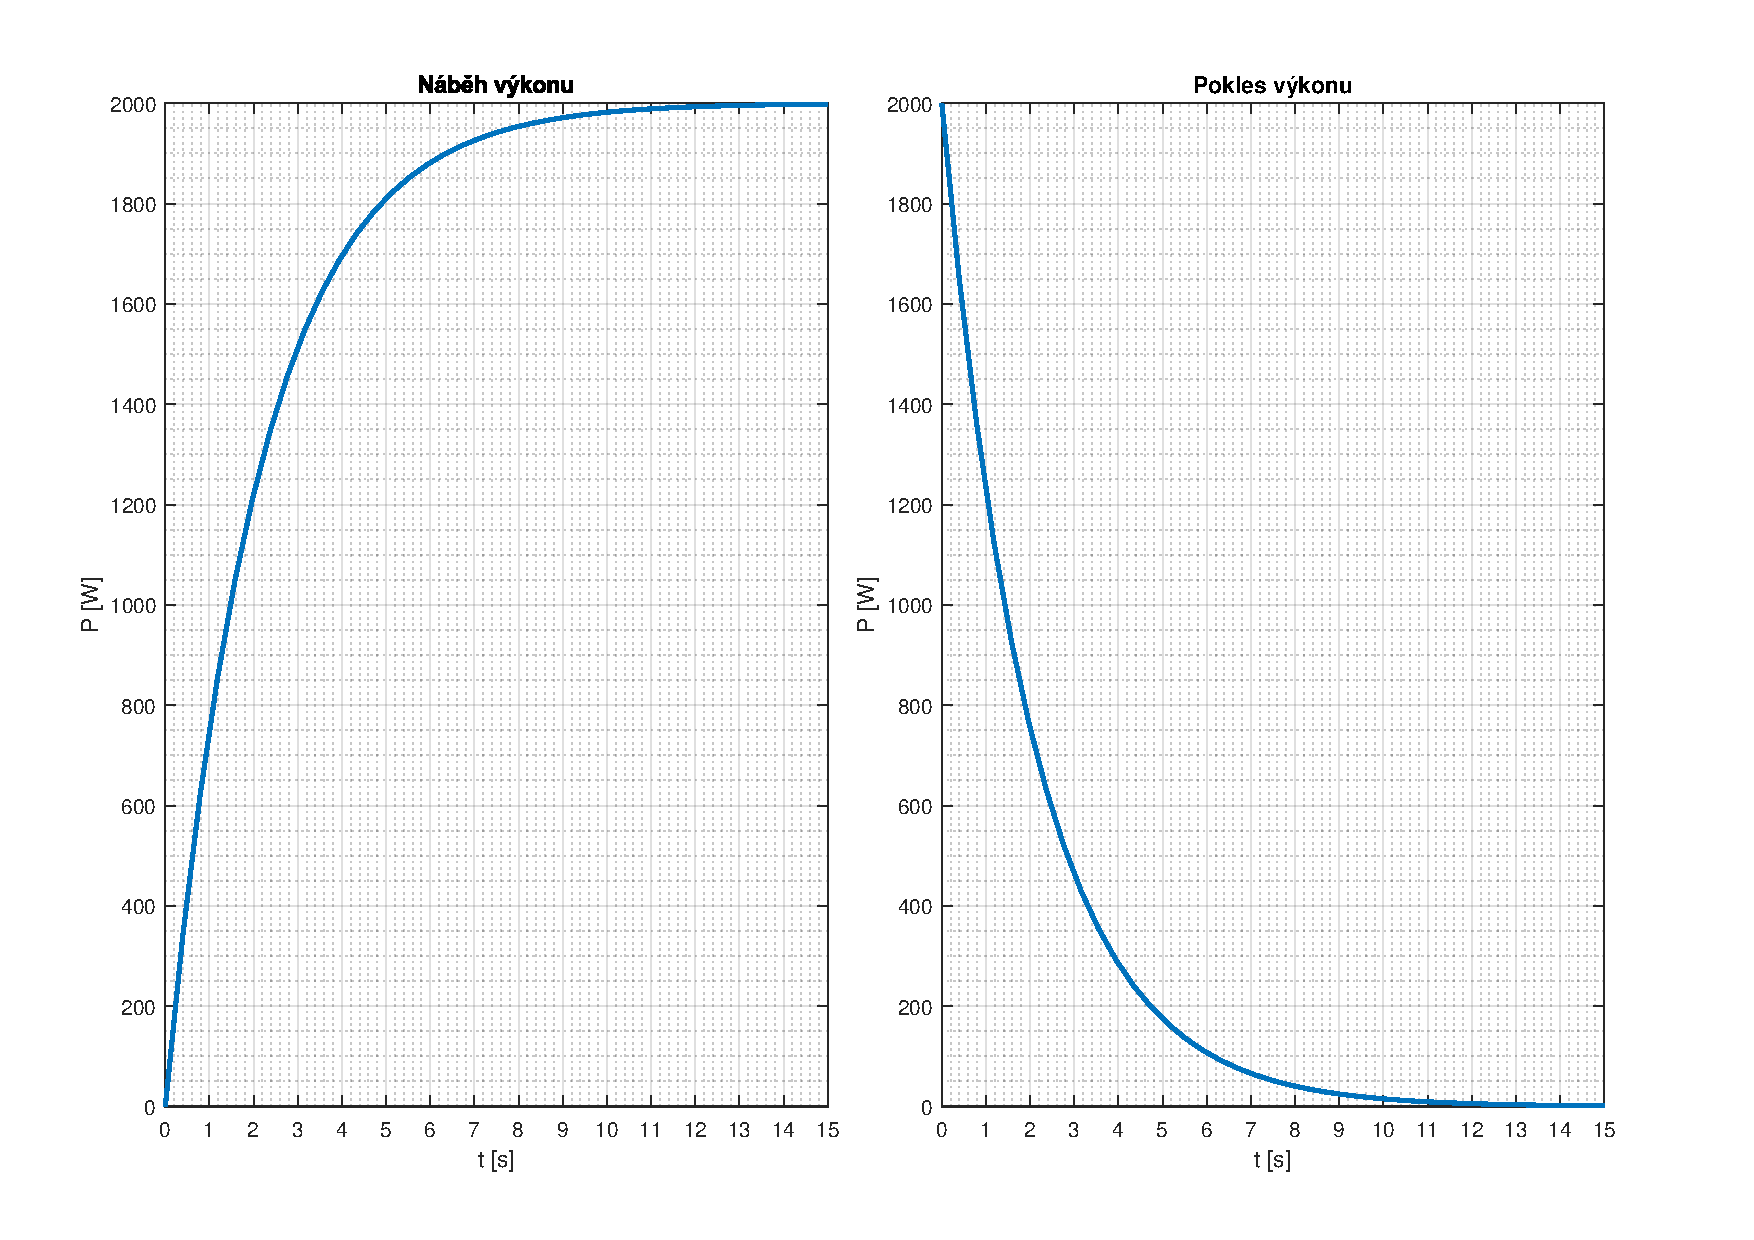
\includegraphics[scale=0.52]{obrazky/simulace_funkce.pdf}
    \end{center}
    \caption[Průběh funkcí pro simulaci]{Průběh funkcí pro simulaci}
    \label{fig:simulace_funkce}
\end{figure}
\noindent Toto funkce bylo potřeba převést do rekurzivní podoby, aby bylo možné je implementovat do funkčního bloku.

\begin{equation}
    y_{RůstTed} = y_{RůstPred} + \frac{ln(1 + k_{Růst} \cdot \Delta t)}{ln(1 + k_{Růst} \cdot T_{Max})} \cdot (y_{Max} - y_{RůstPred}) 
    \label{eq:rust_rekurzivni}
\end{equation}
\begin{equation}
    y_{PoklesTed} = y_{PoklesPred} \cdot e^{k_{Pokles} \cdot \Delta t}
    \label{eq:pokles_rekurzivni}
\end{equation}
\noindent\textit{Kde:}
\begin{itemize}
    \item $y_{RůstTed}$ - nový výkon [W]
    \item $y_{RůstPred}$ - předchozí výkon [W]
    \item $k_{Růst}$ - korekční člen pro pokles [-]
    \item $\Delta t$ - časový krok [s]
    \item $T_{Max}$ - maximální čas růstu výkonu [s]
    \item $y_{Max}$ - maximální výkon [W]
    \item $y_{PoklesTed}$ - nový výkon [W]
    \item $y_{PoklesPred}$ - předchozí výkon [W] \newline
\end{itemize}
\noindent Po vyčtení výkonu topení a klimatizace zbývá vypočítat teplotu v místnosti. Ten se získá součtu aktuální hodnoty teploty a přírůstku podílu působích toků a potřebné energie ke změně teploty (Rov. \ref{eq:energie}). Rovnice pro celkový tepelný tok je dána jako součet tepelných toků ze stran, výkonu topení a klimatizace (působí záporně).
\begin{equation}
    T_{Aktualni} = T_{Predchozi} + \frac{\phi _{Celkovy}}{Q}
    \label{eq:aktualni_teplota}
\end{equation}
\begin{equation}
    \phi _{Celkovy} = \sum_{i=1}^{6} \phi _{Strana_i} + \phi _{Topeni} - \phi _{Klimatizace}
    \label{eq:celkovy_tepelny_tok}
\end{equation}
\noindent\textit{Kde:}
\begin{itemize}
    \item $T_{Aktualni}$ - aktuální teplota [°C]
    \item $T_{Predchozi}$ - předchozí teplota [°C]
    \item $\phi _{Celkovy}$ - celkový tepelný tok [W]
    \item $\phi _{Strana_i}$ - tepelný tok ze strany i [W]
    \item $\phi _{Topeni}$ - tepelný tok z topení [W]
    \item $\phi _{Klimatizace}$ - tepelný tok z klimatizace [W] \newline
\end{itemize}

\noindent Průběh teploty v místnosti je zobrazen na Obr. \ref{fig:simulace_teplota}, kde je demonstrováno chování při běhu topení a klimatizace v horním grafu. Ve spodní části grafu je zase zobrazeno chování teploty bez působení topení a klimatizace. Teplota okolí je v tomto případě nastavená na 21 °C. Z průběhu lze vypozorovat, že se teplota ustálí na teplotu okolí a tudíž, lze považovat model za korektní.
\begin{figure}[!ht]
    \begin{center}
        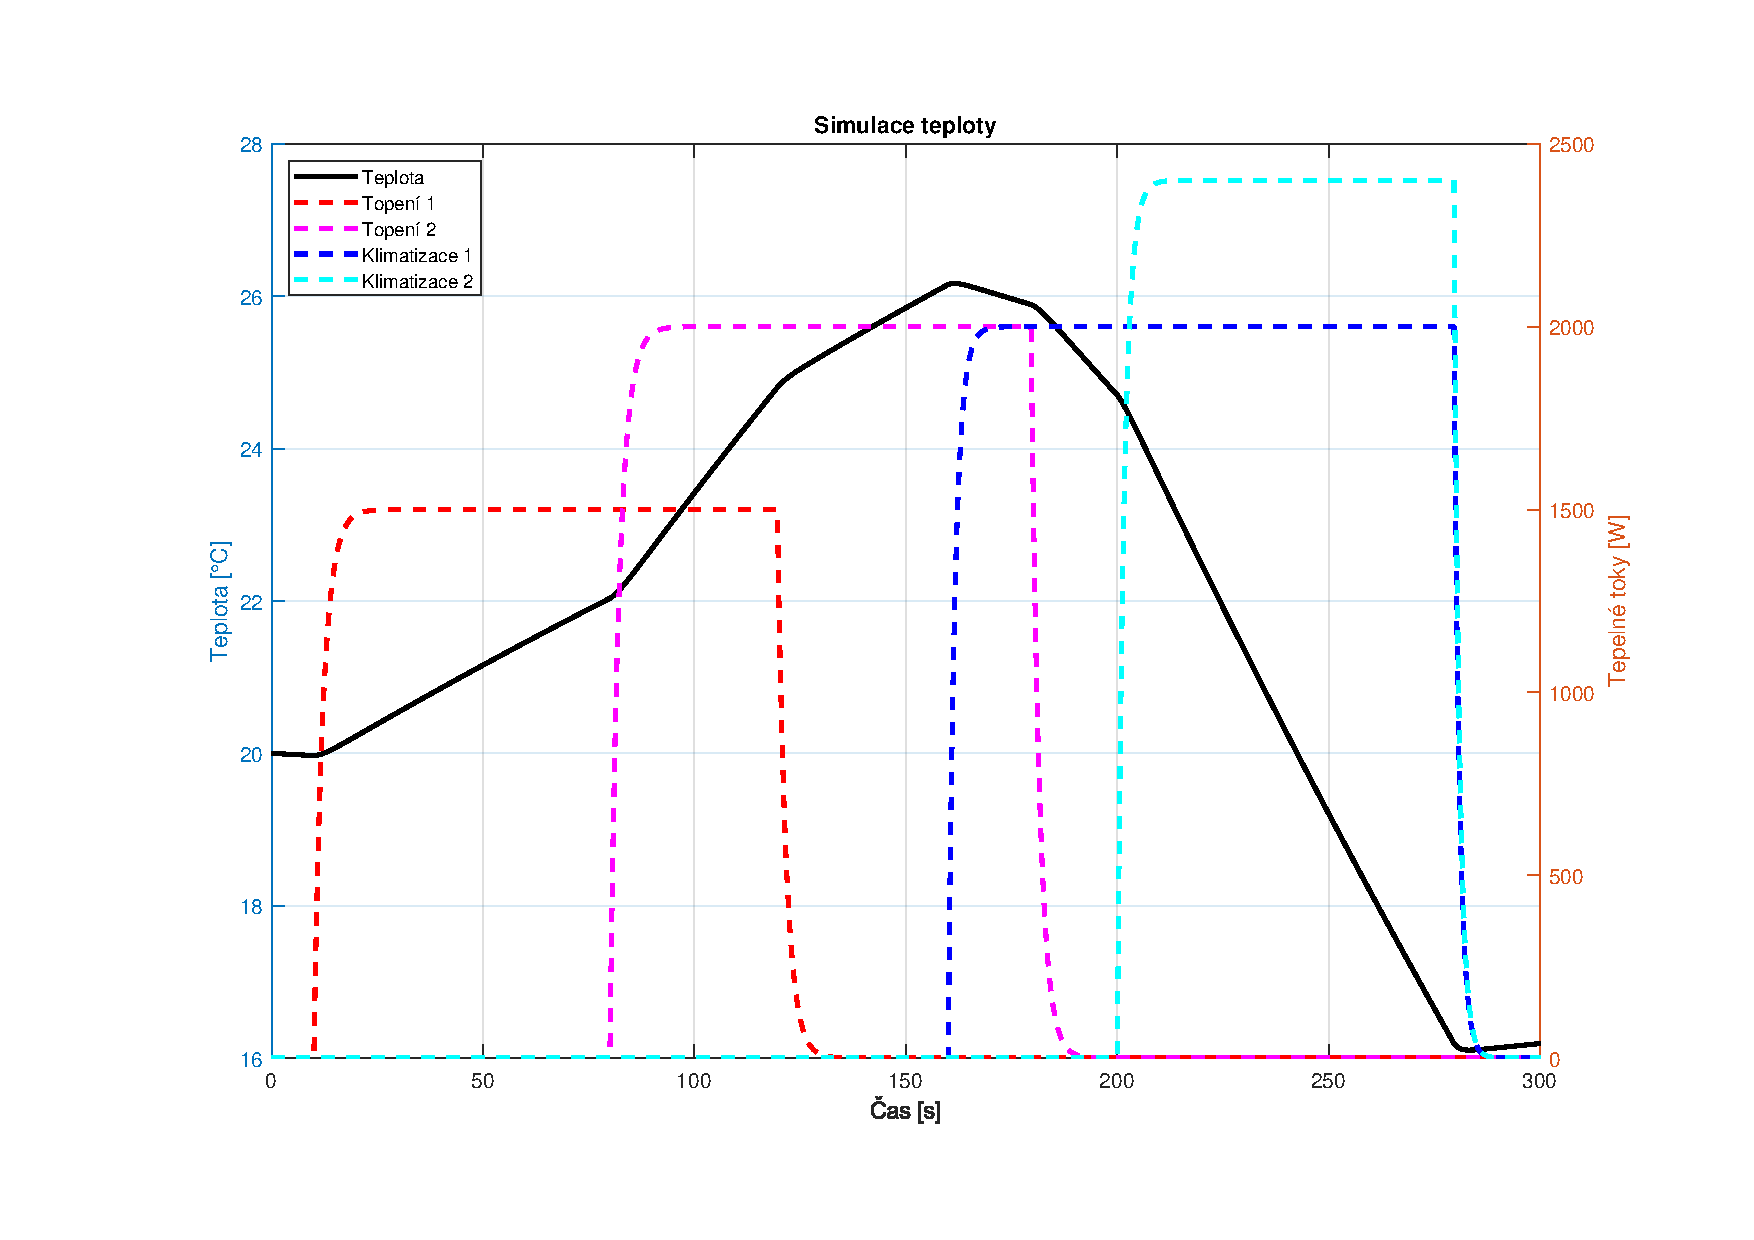
\includegraphics[scale=0.52]{obrazky/simulace_teploty_kuchyne.pdf}
    \end{center}
    \caption[Simulace teploty v místnosti]{Simulace teploty v místnosti}
    \label{fig:simulace_teplota}
\end{figure}

\noindent Tento funkční blok byl použit pro simulaci teploty v obývacím pokoji, kuchyni. Definice tohoto funkčního bloku je zobrazena kvůli své velikosti v příloze číslo 2. Pro venkovní teplotu byl použit signál, který byl napojen na teploměr na panelu. V případě koupelny byla teplota simulována jako sinusoida v rozmezí 18-22 °C a periodou 3 minuty. Tento způsob byl zvolen kvůli absenci teploměru a akčního členu pro řízení teploty. 

\subsubsection{fbLivRoom}
\subsubsection{fbKitch}
\subsubsection{fbBath}
\subsubsection{fbOutz}

\subsection{Komunikace KNX/IP}
\subsection{Komunikace MQTT}
\subsection{Vizualizace}